\chapter{Model Development with TensorFlow/Keras}\label{ch:model}

\section*{Where training ran}\label{sec:2-0}
All model code lives in \file{src/visionguard/} and is driven by \file{scripts/train.py}; every
setting comes from \file{params.yaml} and can be overridden per run
(\cmd{--set train.lr_head=0.0001}). Data preparation ran on my laptop; the training runs ran on a
Google Colab T4 GPU (\file{notebooks/train_colab.ipynb}), which clones the same commit from GitHub
and pulls the same data version with \cmd{dvc pull}, so a run is fully identified by the
\texttt{git\_commit} and \texttt{dvc\_data\_version} tags it logs.

\section{Input pipeline}
\textbf{Stages} (\file{src/visionguard/data.py}, \texttt{make\_dataset}):
\begin{enumerate}
\item \textbf{List}: \texttt{from\_tensor\_slices((paths, labels))} from the split CSV. Reading
the split lists, not the folders, guarantees the same images land in the same split every time.
\item \textbf{Decode + resize} (parallel): \texttt{tf.numpy\_function} calls the shared Pillow
function \texttt{decode\_and\_resize} with \texttt{num\_parallel\_calls=AUTOTUNE}. The output is a
$224\times224\times3$ tensor of raw 0--255 values.
\item \textbf{Cache}: the decoded images are cached in RAM after the first epoch as
\texttt{uint8} (4$\times$ smaller than \texttt{float32}), so JPEG decoding happens once.
\item \textbf{Shuffle} (training only): buffer = whole training set, fixed seed, reshuffled every epoch.
\item \textbf{Batch} (32) and \textbf{augment} (training only, applied to whole batches):
horizontal flip, rotation $\pm$5\%, zoom $\pm$10\%, translation $\pm$5\%, contrast $\pm$10\%.
\item \textbf{Prefetch}: the CPU prepares the next batch while the GPU trains on the current one.
\end{enumerate}
Validation and test data go through the same stages without shuffle and augmentation, so they
are evaluated exactly as they are.

\textbf{Image size.} 224\,px is the resolution MobileNetV2 was pre-trained on, so its filters
see objects at the scale they learned; it also keeps the batch cheap. One experiment uses
160\,px to measure the effect (\cref{sec:3-5}).

\textbf{Aspect ratio.} The default resize \emph{squashes} every image to a square, so a
$1000\times500$ photo is compressed horizontally by 2$\times$ and its aspect ratio is lost. The
alternative (\texttt{resize\_mode: pad}) keeps the ratio and pads with black bars, but then the
amount of padding itself tells the model the original shape, which is one of the shortcuts found
in the EDA. I kept squashing for both classes so the shape signal is neutral.

\textbf{Augmentation choices.} The augmentations change geometry and global contrast but keep
fine texture. I deliberately avoided blur, noise and JPEG re-compression: those destroy the
high-frequency artefacts that distinguish generated images, and could turn an AI image into
something that statistically looks like a camera image while keeping the ``AI'' label.

\autofig{batch_plain}{A training batch after decode + resize, before augmentation.}
\autofig{batch_augmented}{The same batch after the training-time augmentation.}

\section{Baseline CNN from scratch}
\textbf{Architecture} (\file{models.py}, \texttt{build\_baseline}). Every layer has a job:
\begin{itemize}
\item \textbf{Rescaling(1/255)}: maps pixels to $[0,1]$ inside the model, so serving code only
sends raw pixels and cannot forget the scaling.
\item \textbf{4 blocks of Conv2D(3$\times$3) $\rightarrow$ BatchNorm $\rightarrow$ ReLU
$\rightarrow$ MaxPool(2)} with 32, 64, 128, 256 filters: convolutions learn local patterns
(edges, then textures, then parts); doubling filters while halving resolution keeps compute
balanced; BatchNorm normalises activations so training is stable with a higher learning rate
(the conv has \texttt{use\_bias=False} because BN's shift replaces the bias); ReLU adds
non-linearity; pooling gives translation tolerance and grows the receptive field.
\item \textbf{GlobalAveragePooling}: averages each feature map to one number, turning
$14\times14\times256$ into 256 values. Far fewer parameters than \texttt{Flatten} + Dense, which
matters with only a few hundred training images.
\item \textbf{Dropout(0.4)}, \textbf{Dense(64, ReLU)}, \textbf{Dropout(0.2)}: a small
classifier head; dropout randomly zeroes units during training to reduce over-fitting.
\item \textbf{Dense(1, sigmoid)}: one output $p = P(\text{AI}\mid\text{image})$.
\end{itemize}

\textbf{Loss, optimiser, metrics.} Binary cross-entropy is the negative log-likelihood of a
Bernoulli output, the natural loss for one sigmoid unit, and it rewards calibrated probabilities
(which I need, because the threshold is chosen later). Adam with learning rate $10^{-3}$ adapts
per-parameter step sizes and works well without tuning on small CNNs. Metrics: accuracy (easy to
read), ROC-AUC (threshold-free ranking quality), precision and recall of the AI class (the two
error types of \cref{sec:2-5}). Inverse-frequency class weights stop the model from ignoring the
smaller class.

\gentable{baseline_layers}{Baseline CNN: output shape and parameter count per layer (\vgBaselineParams{} parameters).}
\shot{s2_2_summary}{\texttt{model.summary()} of the baseline CNN.}

\section{Transfer learning (MobileNetV2)}
\textbf{Why MobileNetV2.} Its depthwise-separable convolutions give good ImageNet features with
only about 2.3\,M backbone parameters (14\,MB on disk), so it fine-tunes quickly on a small
dataset and runs fast on the CPU-only server. It is loaded with
\cmd{keras.applications.MobileNetV2(include_top=False, weights="imagenet")}: no 1000-class
classifier, just the convolutional feature extractor ending in a $7\times7\times1280$ map.

\textbf{Preprocessing.} MobileNetV2 was trained on pixels scaled to $[-1,1]$
(\texttt{mobilenet\_v2.preprocess\_input} computes $x/127.5-1$). Feeding $[0,1]$ or $[0,255]$
would shift every activation away from what the pre-trained filters expect and destroy the value
of the weights. I put this scaling inside the model as \texttt{Rescaling(1/127.5, offset=-1)},
so the saved model always applies it, in training and in serving. (EfficientNetB0, used in one
experiment, contains its own normalisation and expects raw 0--255, so it gets an identity layer.)

\textbf{Head.} GlobalAveragePooling $\rightarrow$ Dropout(0.3) $\rightarrow$ Dense(1, sigmoid).

\textbf{Stage 1 (frozen backbone).} \texttt{base.trainable = False}; only the head
(1\,281 weights) learns, at learning rate $10^{-3}$. Random head weights produce large
gradients; if the backbone were trainable, those gradients would wreck the pre-trained filters.

\textbf{Stage 2 (last block unfrozen).} Only the layers of MobileNetV2's last inverted-residual
block (\texttt{block\_16}) and the final \texttt{Conv\_1} are made trainable:
\IfFileExists{generated/transfer_unfrozen.tex}{\texttt{block\_16\_expand}, \texttt{block\_16\_expand\_relu}, \texttt{block\_16\_depthwise}, \texttt{block\_16\_depthwise\_relu}, \texttt{block\_16\_project}, \texttt{Conv\_1}, \texttt{out\_relu}}{\vgPending}.
The model is recompiled (required for the change to take effect) with a learning rate 100$\times$
smaller ($10^{-5}$), so the high-level features adapt to generator artefacts without forgetting
ImageNet. BatchNorm layers stay frozen and the backbone is called with \texttt{training=False}:
otherwise BN would replace ImageNet statistics with statistics from batches of 32 images.

\gentable{transfer_trainable}{Trainable weights in each stage.}
\autofig{transfer_stage1_curves}{Stage 1 (frozen backbone): loss and accuracy.}
\autofig{transfer_stage2_curves}{Stage 2 (last block unfrozen, learning rate $10^{-5}$): loss and accuracy.}
\gentable{transfer_layers}{Transfer model, top-level layers (\vgTransferParams{} parameters in total, \vgTransferTrainable{} trainable in stage 2).}

\begin{wrongbox}
In Keras 3, renaming the backbone with \texttt{base.\_name = "backbone"} silently had no effect,
so \texttt{model.get\_layer("backbone")} failed when unfreezing. Passing \texttt{name="backbone"}
to the constructor fixed it.
\end{wrongbox}

\section{Training discipline}
\begin{itemize}
\item \textbf{Seeds}: \cmd{keras.utils.set_random_seed(42)} seeds Python, NumPy and TensorFlow
together; \texttt{PYTHONHASHSEED} is fixed; the split, the shuffle and every augmentation layer
get explicit seeds. (GPU kernels are not bit-exact, so reruns on a GPU can differ in the third
decimal; the seed is logged as a tag on every run.)
\item \textbf{EarlyStopping} on \texttt{val\_loss}, patience 4, \texttt{restore\_best\_weights=True}.
\item \textbf{ModelCheckpoint} on \texttt{val\_loss} with \texttt{save\_best\_only}. One checkpoint
object is shared by both transfer stages, so it keeps the best epoch \emph{across} stages; after
training I reload that file, so the evaluated model is the best one, not the last one.
\item \textbf{ReduceLROnPlateau}: multiplies the learning rate by 0.3 after 2 epochs without
improvement in \texttt{val\_loss}.
\end{itemize}
Best epochs (lowest validation loss): baseline CNN \textbf{epoch \vgBaselineBestEpoch}, transfer
model \textbf{epoch \vgTransferBestEpoch} (counted across both stages).

\autofig{baseline_curves}{Baseline CNN: loss and accuracy, best epoch marked in red.}
\autofig{transfer_curves}{Transfer model, both stages: best epoch in red, start of fine-tuning dotted.}

\yours{Describe what the curves show, e.g.\ whether validation loss flattened before training
loss (over-fitting) and whether stage 2 lowered validation loss further.}

\section{Evaluation}\label{sec:2-5}
\textbf{Which error is worse?} A \emph{false positive} (a real photo called AI-generated) is
worse for this product. VisionGuard would be used to judge whether someone's photo is genuine; a
false accusation harms a real person (a journalist, a seller, a student) and destroys trust in the
tool. A false negative (an AI image passing as real) is bad but is the status quo without the
tool. So I want high \emph{precision} on the AI class, i.e.\ a low false-positive rate.

\textbf{Threshold.} The test set is used once, at the end. The threshold is chosen on the
\emph{validation} predictions: I scan $t\in[0.05,0.95]$ and pick the value that maximises
$F_{\beta}$ with $\beta=0.5$, which weights precision twice as much as recall and therefore
encodes the choice above. Chosen thresholds: baseline \vgBaselineThr, transfer \vgTransferThr.
The threshold is saved with the model (\file{model_meta.json}) and used by the server.

\gentable{model_metrics}{Test-set metrics at the validation-chosen threshold (FPR = real photos called AI).}

\begin{figure}[H]\centering
\begin{subfigure}{0.45\linewidth}\centering
\IfFileExists{figures/auto/baseline_confusion_matrix.png}{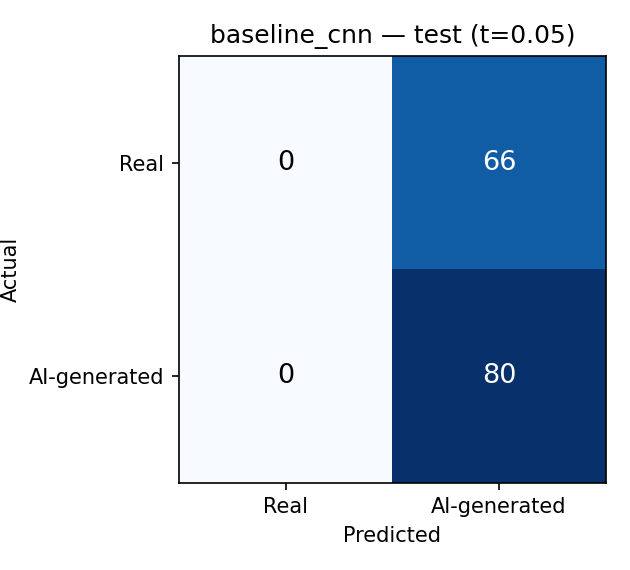
\includegraphics[width=\linewidth]{auto/baseline_confusion_matrix.png}}{\fbox{\parbox[c][3cm][c]{0.9\linewidth}{\centering generated}}}
\caption{Baseline CNN}\end{subfigure}\hfill
\begin{subfigure}{0.45\linewidth}\centering
\IfFileExists{figures/auto/transfer_confusion_matrix.png}{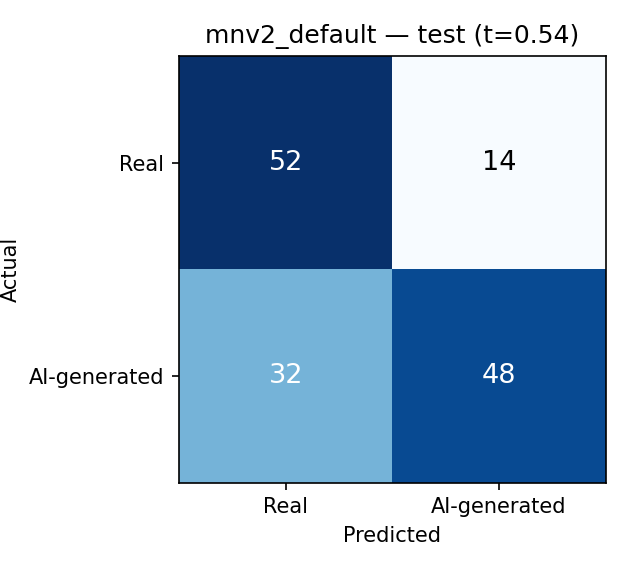
\includegraphics[width=\linewidth]{auto/transfer_confusion_matrix.png}}{\fbox{\parbox[c][3cm][c]{0.9\linewidth}{\centering generated}}}
\caption{MobileNetV2 transfer}\end{subfigure}
\caption{Test confusion matrices.}\label{fig:cms}\end{figure}

\begin{figure}[H]\centering
\begin{subfigure}{0.45\linewidth}\centering
\IfFileExists{figures/auto/baseline_roc_curve.png}{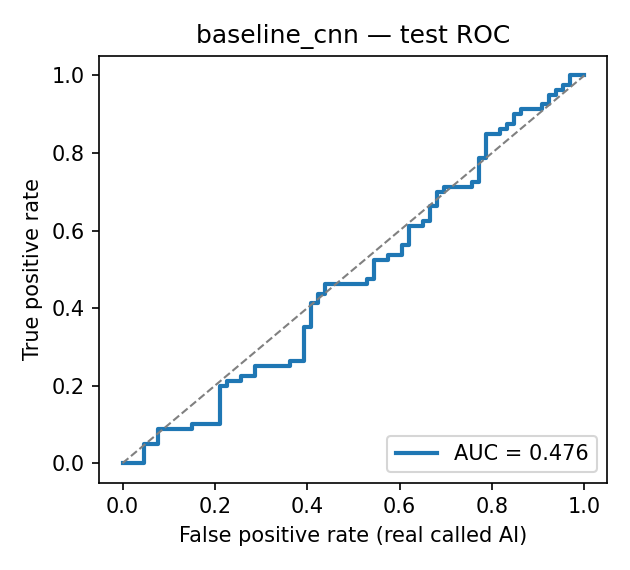
\includegraphics[width=\linewidth]{auto/baseline_roc_curve.png}}{\fbox{\parbox[c][3cm][c]{0.9\linewidth}{\centering generated}}}
\caption{Baseline CNN}\end{subfigure}\hfill
\begin{subfigure}{0.45\linewidth}\centering
\IfFileExists{figures/auto/transfer_roc_curve.png}{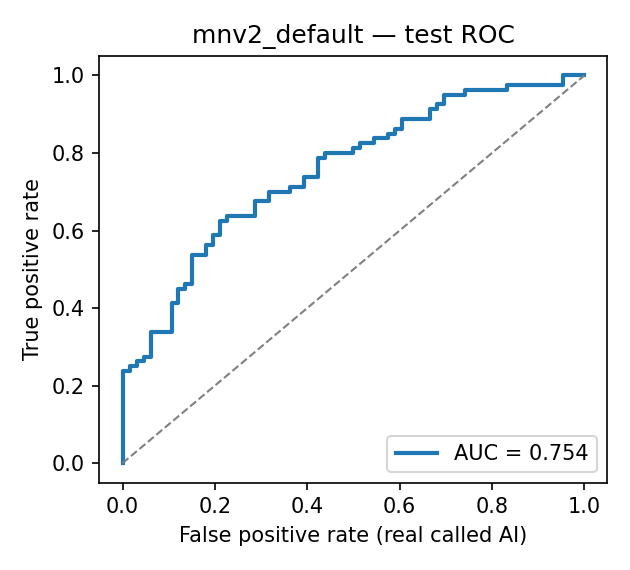
\includegraphics[width=\linewidth]{auto/transfer_roc_curve.png}}{\fbox{\parbox[c][3cm][c]{0.9\linewidth}{\centering generated}}}
\caption{MobileNetV2 transfer}\end{subfigure}
\caption{Test ROC curves.}\label{fig:rocs}\end{figure}

The transfer model reaches test accuracy \vgTransferAccuracy{}, F1 \vgTransferFOne{} and ROC-AUC
\vgTransferRocauc{}, with a false-positive rate of \vgTransferFalsepositiverate{}; the
baseline reaches \vgBaselineAccuracy{}, \vgBaselineFOne{} and \vgBaselineRocauc{} (FPR
\vgBaselineFalsepositiverate{}).

\yours{One or two sentences: which model is better and by how much; is the gap mainly in AUC (ranking)
or at the threshold? Pre-trained features usually win clearly on a dataset this small.}

\section{Error analysis}\label{sec:2-6}
\file{scripts/error_analysis.py} takes the champion's test predictions, keeps the ten most
\emph{confident} mistakes (the most informative ones), and measures simple properties of each:
size, sharpness (variance of an edge filter), colour saturation, grey-scale, aspect ratio and
format. These give each error a testable hypothesis instead of a guess.

\autofig{errors_grid}{The ten most confident test errors (true label, prediction, $p(\text{AI})$, size).}
\gentable{errors}{Measured cues and hypothesis per error.}

\yours{Look at each of the 10 images and confirm or correct its hypothesis (e.g.\ watermark,
painting style, text in the image, heavy JPEG artefacts, a real photo of a CGI scene). Note any
pattern, e.g.\ ``most false positives are smooth, studio-lit portraits''.}

\section{Tool lab: Keras Tuner}
\subsection*{Toy part}
\file{labs/tuner_toy.py} tunes a one-hidden-layer network on Fashion-MNIST with
\textbf{Hyperband}: number of units $\in\{32,\dots,512\}$ and learning rate
$\in\{10^{-2},10^{-3},10^{-4}\}$. Hyperband trains many configurations for a few epochs,
keeps the best third, trains those longer, and repeats, so most of the budget goes to promising
settings. \cmd{tuner.get_best_hyperparameters()} returns the winner.
\gentable{tuner_toy}{Toy tuner: best trials on Fashion-MNIST (validation accuracy).}
\shot{s2_7_toy_tuner}{Toy tuner results summary.}

\subsection*{Applied to VisionGuard}
\file{scripts/tune.py} defines a \texttt{HyperModel} whose \texttt{fit()} reproduces the two-stage
training inside each trial and searches the head learning rate (log-uniform
$10^{-4}$--$3\cdot10^{-3}$), dropout (0.1--0.5) and how many backbone layers to unfreeze
$\in\{0, 11\ (\text{last block}), 30, 60\}$ with \textbf{RandomSearch}, \vgTunerTrials{} trials,
objective validation loss. Every trial is also logged to MLflow as a nested run.

\gentable{tuner_trials}{VisionGuard tuner trials, best first.}
\autofig[0.95]{tuner_effects}{Validation loss of each trial against each hyper-parameter.}
\gentable{tuner_effects}{Effect size: spread of mean validation loss across the levels of each hyper-parameter.}
\shot{s2_7_tuner}{Tuner search output for VisionGuard.}

Best trial: learning rate \vgTunerBestLr, dropout \vgTunerBestDrop, \vgTunerBestUnfrozen{}
unfrozen layers (validation loss \vgTunerBestLoss). The hyper-parameter with the largest effect
was \textbf{\vgTunerMostImportant}.

\yours{One sentence on why that hyper-parameter mattered most (e.g.\ the learning rate controls
whether the new head converges in a few epochs; unfreezing many layers on ~600 images over-fits).}

\textbf{Why the best validation score can over-fit the validation set.} The tuner looks at the
validation loss of every trial and keeps the minimum. With many trials, some configurations score
well partly by luck on this particular, small validation set (a ``winner's curse''): selection
itself fits noise in the validation data, so the best score is an optimistic estimate. That is
why the final numbers come from the untouched test set, used once, and why a clearly simpler
setting within noise of the best is a reasonable choice.

\section*{Bonus: Grad-CAM}
\autofig{gradcam}{Grad-CAM heat maps: top row correct predictions, bottom row errors. Red = regions that pushed $p(\text{AI})$ up.}
Grad-CAM takes the gradient of the output with respect to the last convolutional feature map,
averages it per channel to get channel weights, and shows the weighted sum of the feature maps as
a heat map.

\yours{Comment on what the model looks at, e.g.\ skin/hair texture and backgrounds for AI
portraits (where generators leave smooth, repetitive texture), versus edges of objects or
watermark areas in the errors.}
